%
% robertson.tex -- Funktion S_\kappa(r) 
%
% (c) 2017 Prof Dr Andreas Müller, Hochschule Rapperswil
%
\documentclass[tikz]{standalone}
\usepackage{times}
\usepackage{txfonts}
\usepackage{pgfplots}
\usetikzlibrary{arrows,intersections}
\begin{document}
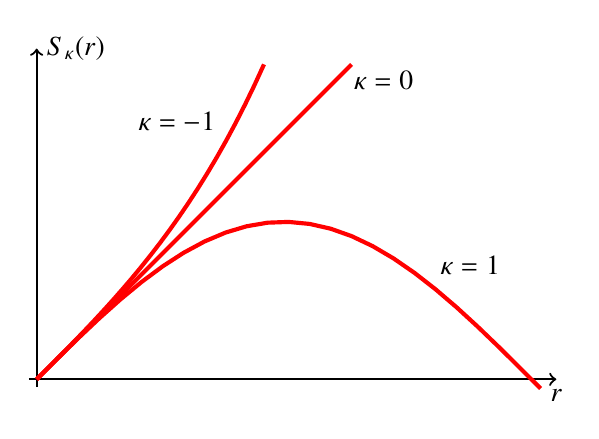
\begin{tikzpicture}[thick,scale=2]
\coordinate (O) at (0,0);
\draw[->] (-0.05, 0   )--(3.3,0  ) coordinate[label = {below:$r$}];
\draw[->] ( 0,   -0.05)--(0,  2.1) coordinate[label = {right:$S_\kappa(r)$}];
\draw[red,domain=0:3.2,line width=1.5] plot (\x,{sin(180 * \x / 3.1415)});
\draw[red,domain=0:2,line width=1.5]   plot (\x,\x);
\draw[red,domain=0:1.4436,line width=1.5] plot (\x,{sinh(\x)});
\node at (2.5, 0.59847) [above right] {$\kappa=1$};
\node at (1.2, 1.5095) [above left] {$\kappa=-1$};
\node at (1.9, 1.9) [right=1mm] {$\kappa=0$};
\end{tikzpicture}
\end{document}


